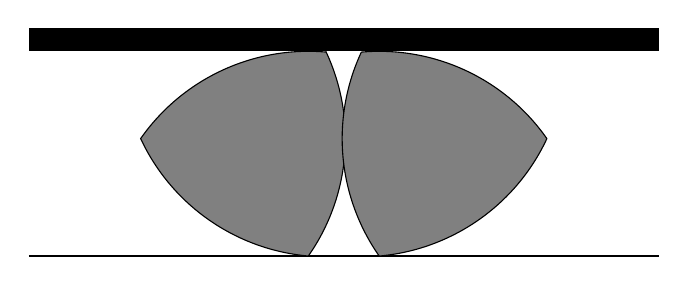
\begin{tikzpicture}
% top bar (thick black plate)
\fill[black] (0,2.6) rectangle (8,2.9);
% bottom line (ground)
\draw[thick] (0,0) -- (8,0);
% Both rollers are true Reuleaux triangles of constant width 2.6
% (= plate gap): three 60-degree arcs, each centered on the opposite
% vertex, radius 2.6. Bottom vertex rests on the ground line, top arc
% is tangent to the top plate.
% left roller: bottom vertex at (3.55,0), axis tilted 25 deg to the left
% vertices: V1=(3.55,0)  V2=(3.777,2.590)  V3=(1.420,1.491)
\filldraw[fill=gray,draw=black]
  (3.777,2.590) arc[start angle=85,  end angle=145, radius=2.6]
                arc[start angle=205, end angle=265, radius=2.6]
                arc[start angle=-35, end angle=25,  radius=2.6]
  -- cycle;
% right roller (mirror image): bottom vertex at (4.45,0), tilted 25 deg right
% vertices: V1=(4.45,0)  Va=(6.580,1.491)  Vb=(4.223,2.590)
\filldraw[fill=gray,draw=black]
  (6.580,1.491) arc[start angle=35,  end angle=95,  radius=2.6]
                arc[start angle=155, end angle=215, radius=2.6]
                arc[start angle=-85, end angle=-25, radius=2.6]
  -- cycle;
\end{tikzpicture}
